\documentclass[a4paper,twoside, openright,12pt]{report}
\usepackage{psfrag,amsbsy,graphics,float}
\usepackage[dvips]{graphicx, color}
\usepackage[latin1]{inputenc}
\usepackage{verbatim} 
\usepackage{appendix}

% MY CHANGE
%\usepackage[bookmarksnumbered=true]{hyperref} 

\usepackage[bookmarks=true,colorlinks=true,       % false: boxed links; true: colored links
    linkcolor=black,          % color of internal links
    citecolor=black,        % color of links to bibliography
    filecolor=black,      % color of file links
    urlcolor=black           % color of external links
]{hyperref}
 

%%% Stand 14.09.2007
%%% erstellt von Marion Sobotka
%%% marion.sobotka@tum.de
%%% last changes: 14.01.09


%_______Kopf- und Fu�zeile_______________________________________________________
\usepackage{fancyhdr}
\pagestyle{fancy}
%um Kopf- und Fu�zeile bei chapter-Seiten zu reaktivieren
\newcommand{\helv}{%
   \fontfamily{phv}\fontseries{a}\fontsize{9}{11}\selectfont}
\fancypagestyle{plain}{	
	\fancyfoot{}% keine Fu�zeile
	\fancyhead[RE]{\helv\leftmark}% Rechts auf geraden Seiten=innen; in \leftmark stehen \chapters
	\fancyhead[LO]{\helv\rightmark}% Links auf ungeraden Seiten=au�en;in \rightmark stehen \sections
	\fancyhead[RO,LE]{\thepage}}%Rechts auf ungeraden und links auf geraden Seiten
%Kopf- und Fu�zeile f�r alle anderen Seiten
\fancyfoot{}
\fancyhead[RE]{\helv\leftmark}
\fancyhead[LO]{\helv\rightmark}%alt:\fancyhead[LO]{\itshape\rightmark}
\fancyhead[RO,LE]{\thepage}
%________________________________________________________________________________


%_Definieren der R�nder und L�ngen__________
\setlength{\textwidth}{15cm}
\setlength{\textheight}{22cm}
\setlength{\evensidemargin}{-2mm}
\setlength{\oddsidemargin}{11mm}
\setlength{\headwidth}{15cm}
\setlength{\topmargin}{10mm}
\setlength{\parindent}{0pt} % Kein Einr�cken beim Absatz!!
%___________________________________________


%_______Titelseite__________________________________________
\begin{document}
\pagestyle{empty}
\enlargethispage{4.5cm} %Damit das Titelbild weit genug unten ist!
\begin{center}
\phantom{u}
\vspace{0.5cm}
\Huge{\sc Numerical Test Rig for Large-Scale and Interconnected Dynamical
Systems}\\
\vspace{1.5cm}
                                 \large{submitted\\
				  Project Laboratory\\
				  Networked and Cooperative Control\\
			  %DIPLOMARBEIT\\%/STUDIENARBEIT/MASTERRBEIT/BACHELORARBEIT\\ 
                               %            von\\
                              %  \large{Zwischenbericht zur\\
			%DIPLOMARBEIT/STUDIENARBEIT/MASTERARBEIT/
					   % BACHELORARBEIT\\ 
					   by         

						
					\begin{tabular}{c c}
					    \vspace{0.4cm} & \vspace{0.4cm} \\
					 cand. ing. Francisco Llobet& cand. ing. Jose Rivera  \\
						\vspace{0.5cm} & \vspace{0.5cm}\\
					born on July 9, 1985 & born on December 18, 1986\\
					resident: & resident:\\
					Briennerstr. 39& Amalienstr. 87\\
					80333 M\"{u}nchen & 80799 M\"{u}nchen  
					\end{tabular}

					                           
					%Tel.: +49\,176\,233\,14721\\
					\vspace{1.5cm}
					Institute of\\
					Automatic Control Engineering\\
					Technische Universit\"{a}t M\"{u}nchen\\
					\vspace{0.3cm}
					Univ.-Prof. Dr.-Ing./Univ. Tokio Martin Buss\\
                                        Univ.-Prof. Dr.-Ing. Sandra Hirche}
\end{center}
\vspace{2.5cm}
\begin{tabular}{ll}
Supervisor: & F. Deroo, S. Erhart, A. Gusrialdi, H. Mangesius  \\
Beginn: & 09.05.2011  \\
Submitted &  04.07.2011 \\
\end{tabular}
%____________________________________________________________

\newpage

%_______Abstract_____________________________________________
\topmargin5mm
\textheight220mm
\pagenumbering{arabic}
\phantom{u}
\begin{abstract}
The goal of this project was to develop a test rig for large-scale and interconnected dynamical systems. The result is
MTIDS or Matlab Toolbox for Interconnected Dynamical Systems, which is a mash-up that wraps different toolboxes used for graph analysis and 
dynamic systems simulation together. MTIDS allows the definition and analysis of graphs, where each node has a specific dynamic assign to it. 
The template based design of nodes' dynamics allows great flexibility for the creation of complex interconnected dynamical systems with the 
possibility of implementing clusters/layers. MTIDS is an open-source project under the GNU GPL v2 license. This document presents a general description 
of MTIDS and instructions for its use.    
%\vspace{2cm}
% \begin{center}
% \normalsize \textbf{Zusammenfassung}\\
% \end{center}
% Dieser Hauptseminar besch\"{a}ftigt sich mit der Methode der getriggerten Optimierung. Dabei wird besonderen Focus auf die m\"{o}glichen Anwendungen f\"{u}r Energiesystemen gesetzt.
% Als erstes wird eine Analyse der Methode in ihre genaralisierte Form f\"{u}r das NUM (Netzwerk Nutzen Maximirung) Problem durchgef\"{u}hrt. Als zweites wird ihre Anwendung an das OPF (Optimale Leistungsfluss) in Energienetzen evaluiert. Als letztes werden
% verbesserungs Vorschl\"{a}gen und weitere Anweundungen in Energiesystemen diskutiert.  
\end{abstract}
%____________________________________________________________

\newpage

%_______Widmung_______________________________________________
\phantom{u}
\phantom{1}\vspace{6cm}
\begin{center}
%Hier die Widmung oder leer lassen
\end{center}
%_____________________________________________________________



\pagestyle{fancy}

%_________Inhaltsverzeichnis__________________________
\tableofcontents 
%_____________________________________________________




%_________Einleitung__________________________________
\chapter{Introduction} \label{chapter1}

In this first Chapter the motivation behind the MTIDS project is explained and the project's goal and framework is presented.

\section{Motivation}
Large-scale interconnected dynamical system are everywhere: biological systems, power and water systems, the brain neurons, 
social interaction networks, economic markets, etc. In a canonical form all of this systems can be thought as a bunch of nodes with local dynamics 
that interact with each other, e.g. a graph. Different topologies of the graph, may lead to different behavior. An example of various 
large scale interconnected systems can be seen in Figure \ref{largePic}. 


\begin{figure}[htb]
\centering
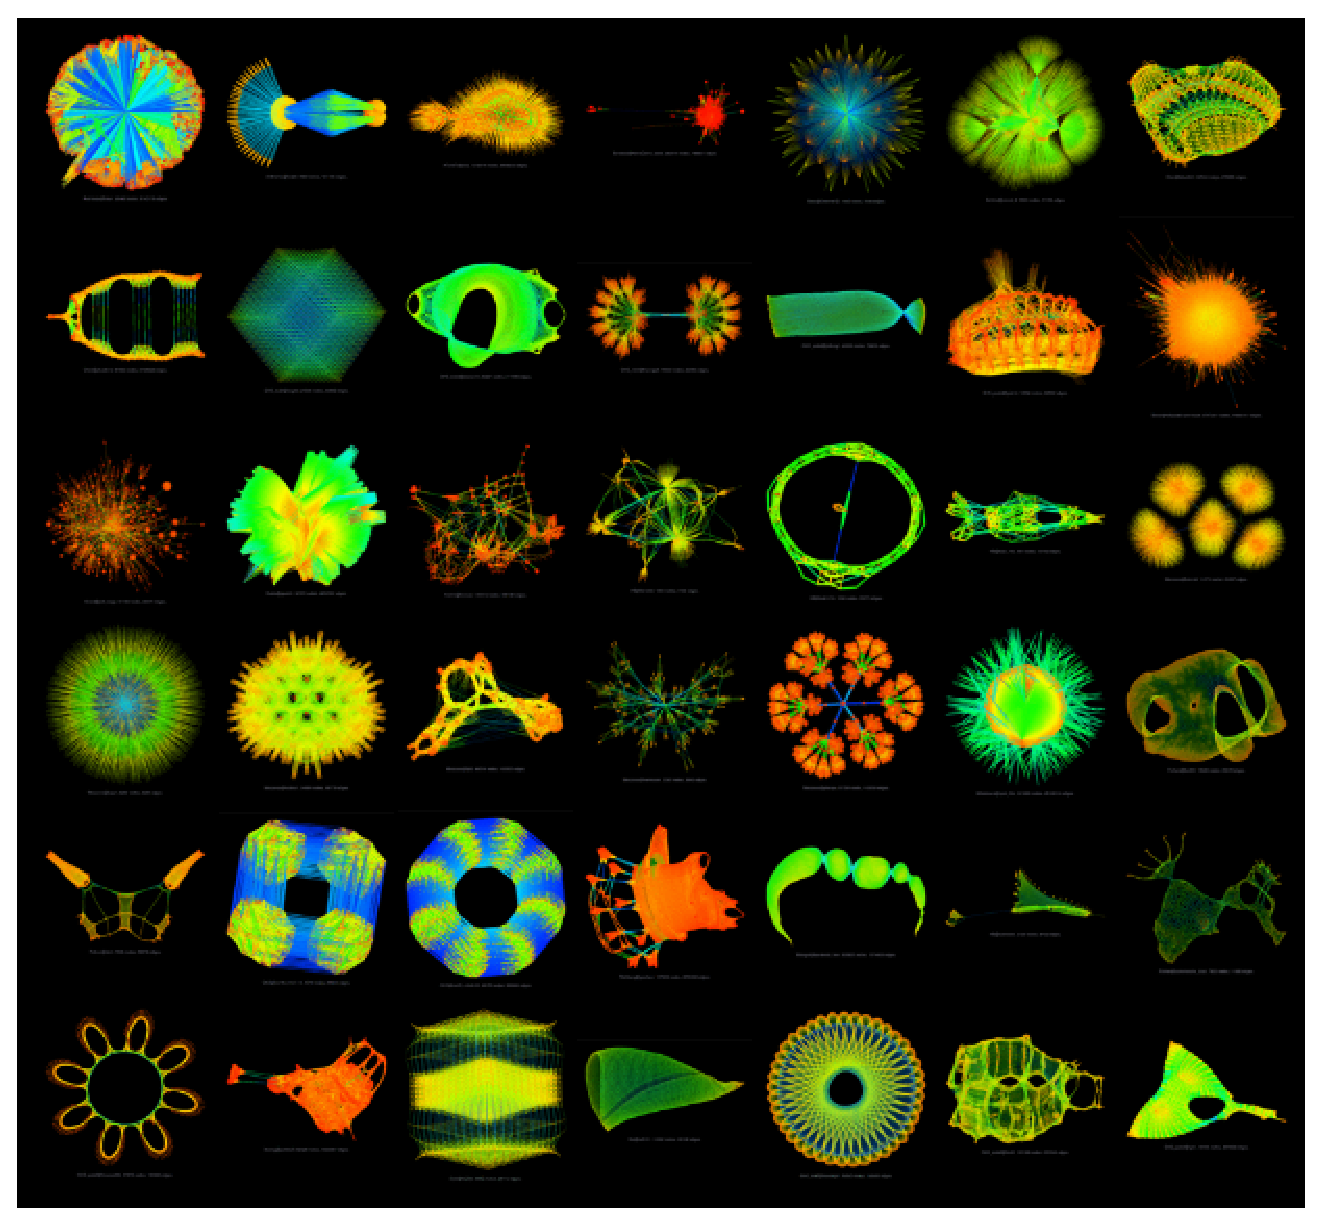
\includegraphics[width=0.5\textwidth]{pics/complex.eps}
\caption[Example of large-scale systems]{Visualization of various large scale systems using the sfdp algorithm $\copyright$ Dr. Yifan Hu of AT\&T Labs}
\label{largePic}
\end{figure}

There are many tools available for the analysis of interconnected dynamical systems, for example in power systems you have PSSE and Power Factory. However,
this simulation programs are normally very system specific and in most cases it takes a long time to learn how to use them correctly. 
The difficulties are specially noticed while
testing control concepts, where small changes on the topology of the grid or control concept could lead to a painful redesign of your simulation set up. 
You may actually end up spending the most of your time in the implementation of a simulation. A more general and 
easy to use solution for the simulation of interconnected dynamical systems is needed.




\section{Idea and Goal}

\textbf{MTIDS} (Matlab Toolbox for Interconnected Dynamical Systems) is a project that aims to design an easy 
to use and flexible toolbox to make the simulation of large scale dynamical systems easier for students and researchers. 
The \textbf{goal} is to produce a mash-up that wraps different toolboxes used for graph analysis and 
dynamic systems simulation together into a framework.  


\begin{figure}[htb]
\centering
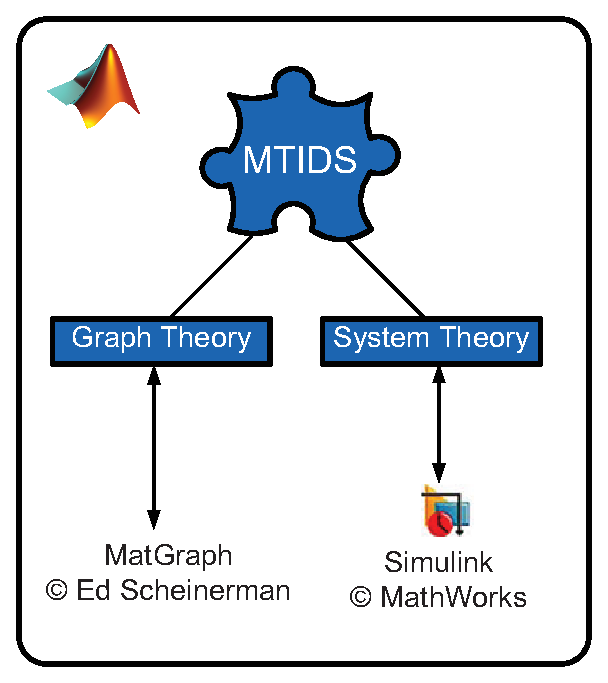
\includegraphics[width=0.5\textwidth]{pics/mtidsStructure.eps}
\caption[MTIDS idea]{MTIDS: Matlab Toolbox for Interconnected Dynamical Systems}
\label{mtidsFig}
\end{figure}

As we can see in Figure \ref{mtidsFig} MTIDS runs in the MATLAB environment and is basically a GUI that allows the interaction of tools used in graph theory 
and control theory.  For graph theory we use Matgraph a toolbox design by Prof. Scheinerman of the John Hopkins University and for dynamical simulations
we use Simulink. 

\section{Framework}

The current framework of MTID is made out of three basic components. A GUI (\textbf{mtids.m}) an export to simulink function (\textbf{exportSimulink.m}) and
an import from Simulink function (\textbf{importSimulink.m}).\\

 

\begin{figure}[htb]
\centering
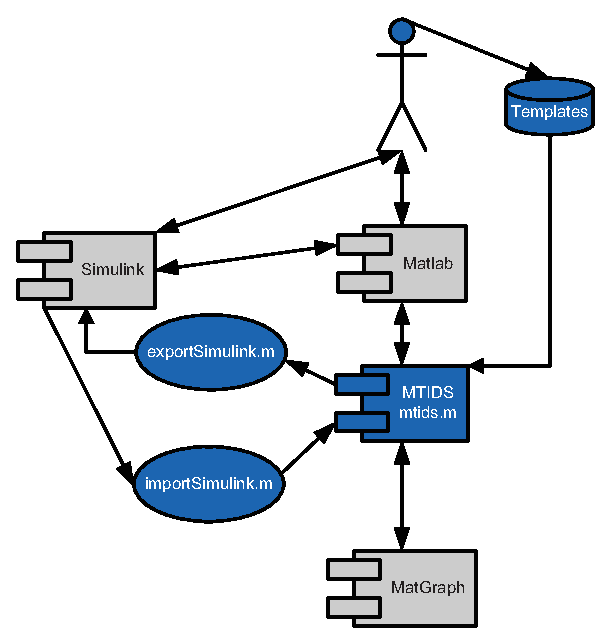
\includegraphics[width=0.5\textwidth]{pics/uml.eps}
\caption[MTIDS components]{MTIDS: Components diagram}
\label{componentsFig}
\end{figure}

In Figure \ref{componentsFig} we can see that the most important component is the user, specially its head. The better you are at producing templates
and interacting with matlab and simulation the more functional MTIDS is going to be for you.
In a nutshell MTIDS works as follows:
\begin{itemize}
\item GUI (mtids.m) runs inside Matlab
\item GUI interacts with Matgraph: create, modify and visualize graphs  
\item System Inteconnector (SI): exportSimulink.m and importSimulink.m called from GUI to interact with Simulink
\item Templates done by User in Matlab/Simulink.
\item Simulations done in Simulink
\end{itemize}
%  
% 
% The GUI (mtids.m) runs inside matlab. The UI interacts 
% with Matgraph to create, modify and visualize graphs. The ystem Inteconnector (SI) compose of the functions exportSimulink.m and importSimulink.m are
% called from GUI to interact with Simulink. The user can define the nodes dynamic by building custom templates in Matlab/Simulink. The simulations are
% ultimately done in Simulink.

%%%%%%%%%%%%%%%%%%%%%%%%%%%%%%%%%%%%%%%%%%%%%%%%%%%%%% GRAPH
\chapter{Graph Theory}\label{chapter2}



%_%%%%%%%%%%%%%%%%%%%%%%%%%%%%%%%%%%%%%%%%%%%%%%%%%%%%%%%%%%%%%%%%%%%%%%%%%%%%%%%%%%%%%%%%%% SYSTEM_____________________________________
\chapter{System Theory}\label{chapter3}

In this Chapter we explain the design and simulation capabilities that MTIDS offers for interconnected dynamical systems.

\section{MTIDS Concepts}
\subsection{Nodes and connections}
\subsubsection{Node:}
Each node represents a subsystem . Each node has to have a unique label, Removing or adding a node changes the numbering of a node. 
\subsubsection{Connections:}
Any connection made inside MTIDS is bidirectional and unweighted. Removing a node removes all connections coming from and to it.

\section{Export to Simulink}\label{exportToSimulink}
In order to export the model created in the MTIDS GUI to simulink: \textbf{Simulation $\rightarrow$ Export to Simulink...} (see Figure \ref{exportFig})

\begin{figure}[htb]
\centering
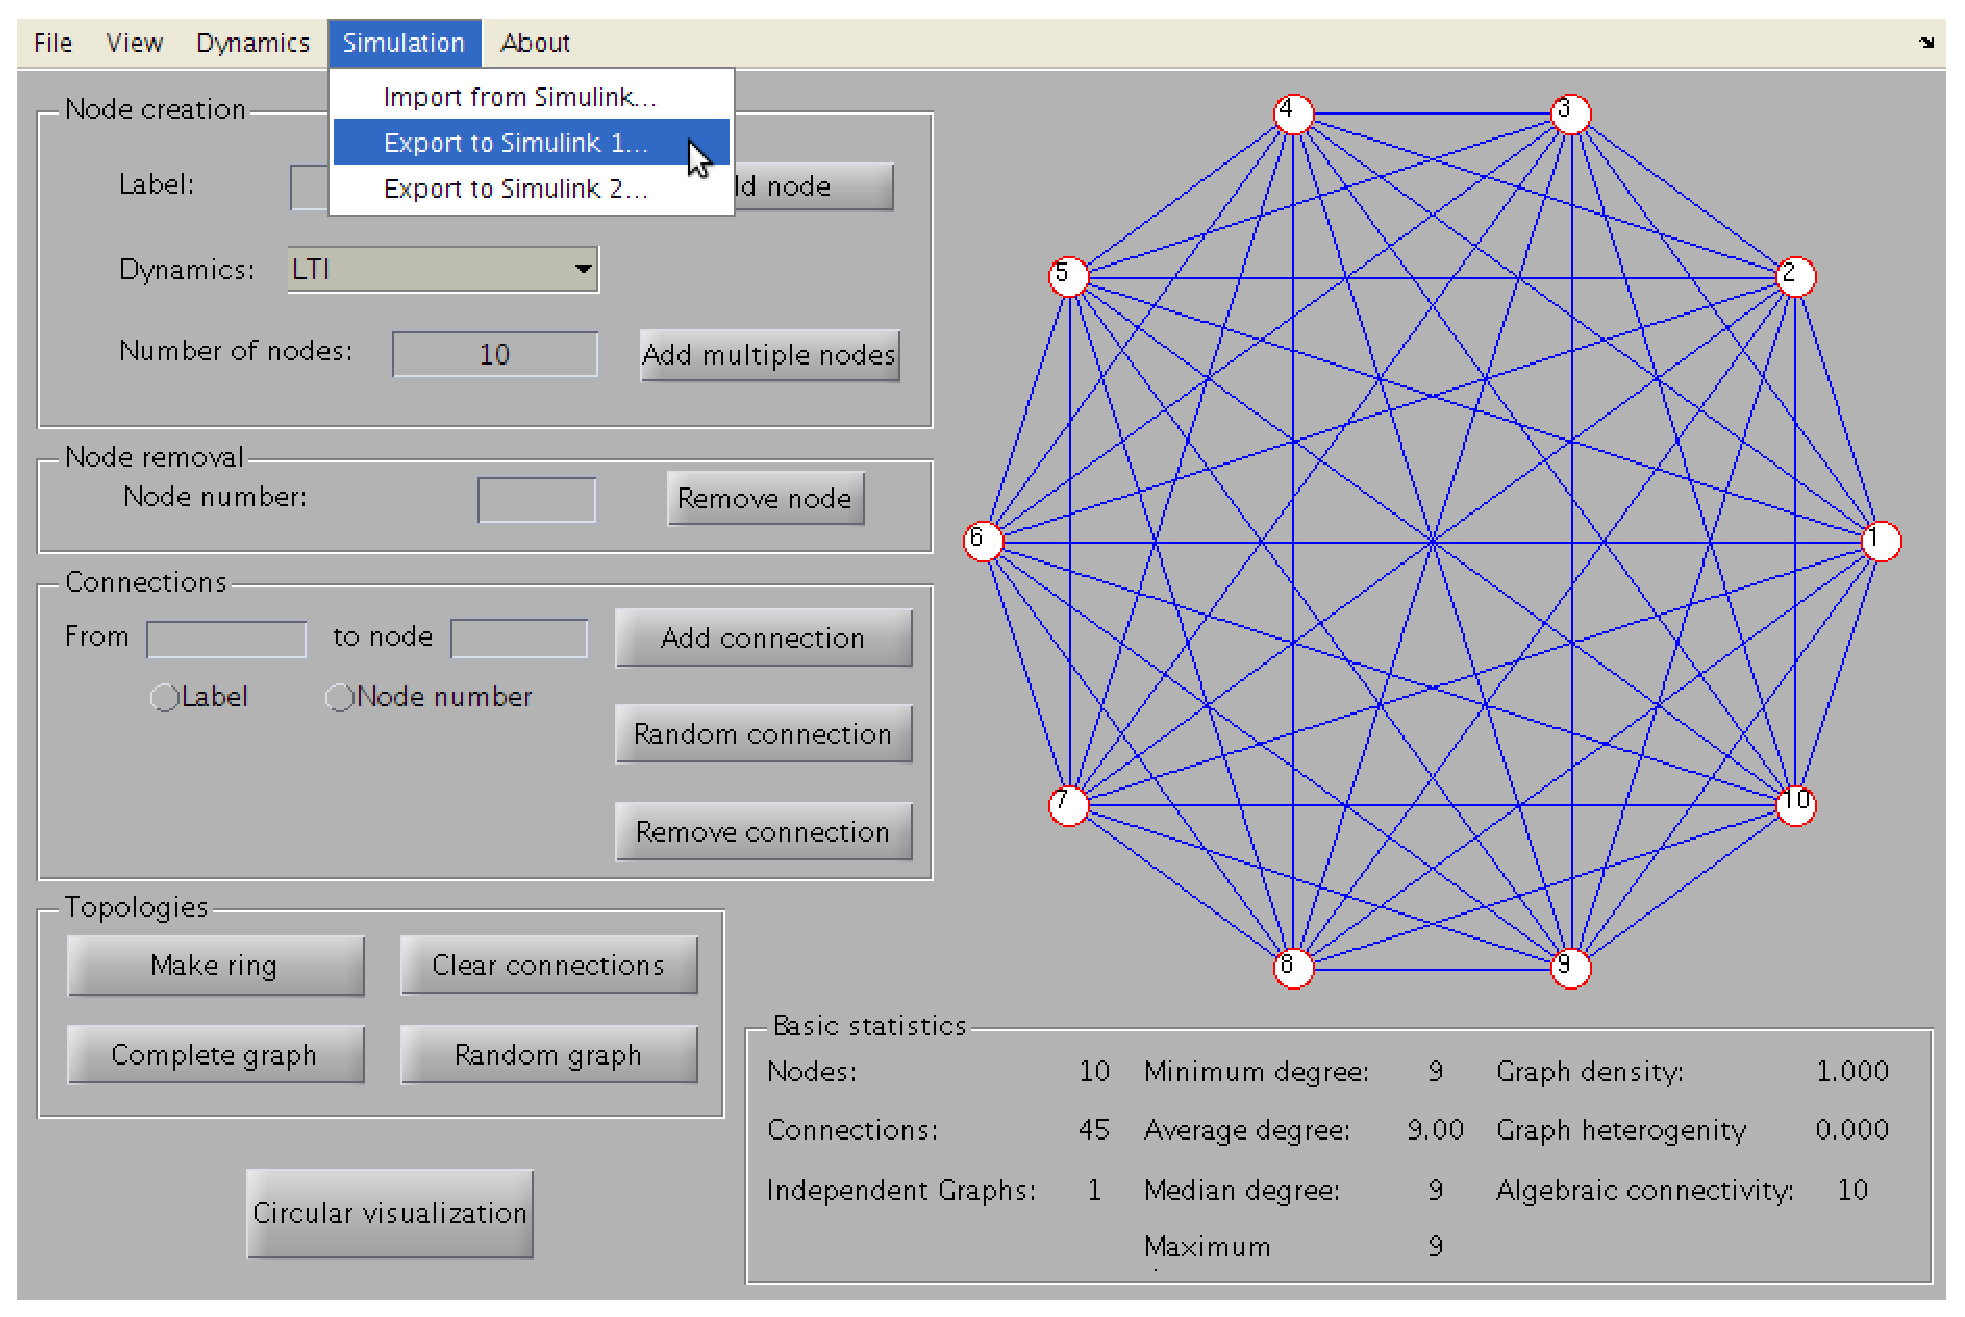
\includegraphics[width=0.8\textwidth]{pics/screenExport.eps}
\caption[MTIDS export to Simulink]{MTIDS: export model to Simulink. Example is a complete graph with 10 LTI nodes. }
\label{exportFig}
\end{figure}

The MTIDS GUI then calls the function exportSimulink.m which builds a Simulink model based with the following information:
\begin{itemize}
 \item name: Model name
 \item template:  list of nodes' dynamics templates 
\item templateList: List of templates that are availible in mtids
\item A: Adjacense matrix,
\item xy: Position of the nodes
 \item labs: List of nodes' names
\end{itemize}
 
The result is a Simulink model in the MTIDS format. To adjust the size of the model to the Simulink window size: \textbf{View $\rightarrow$ Fit System To View}
% 

\begin{figure}[htb]
\centering
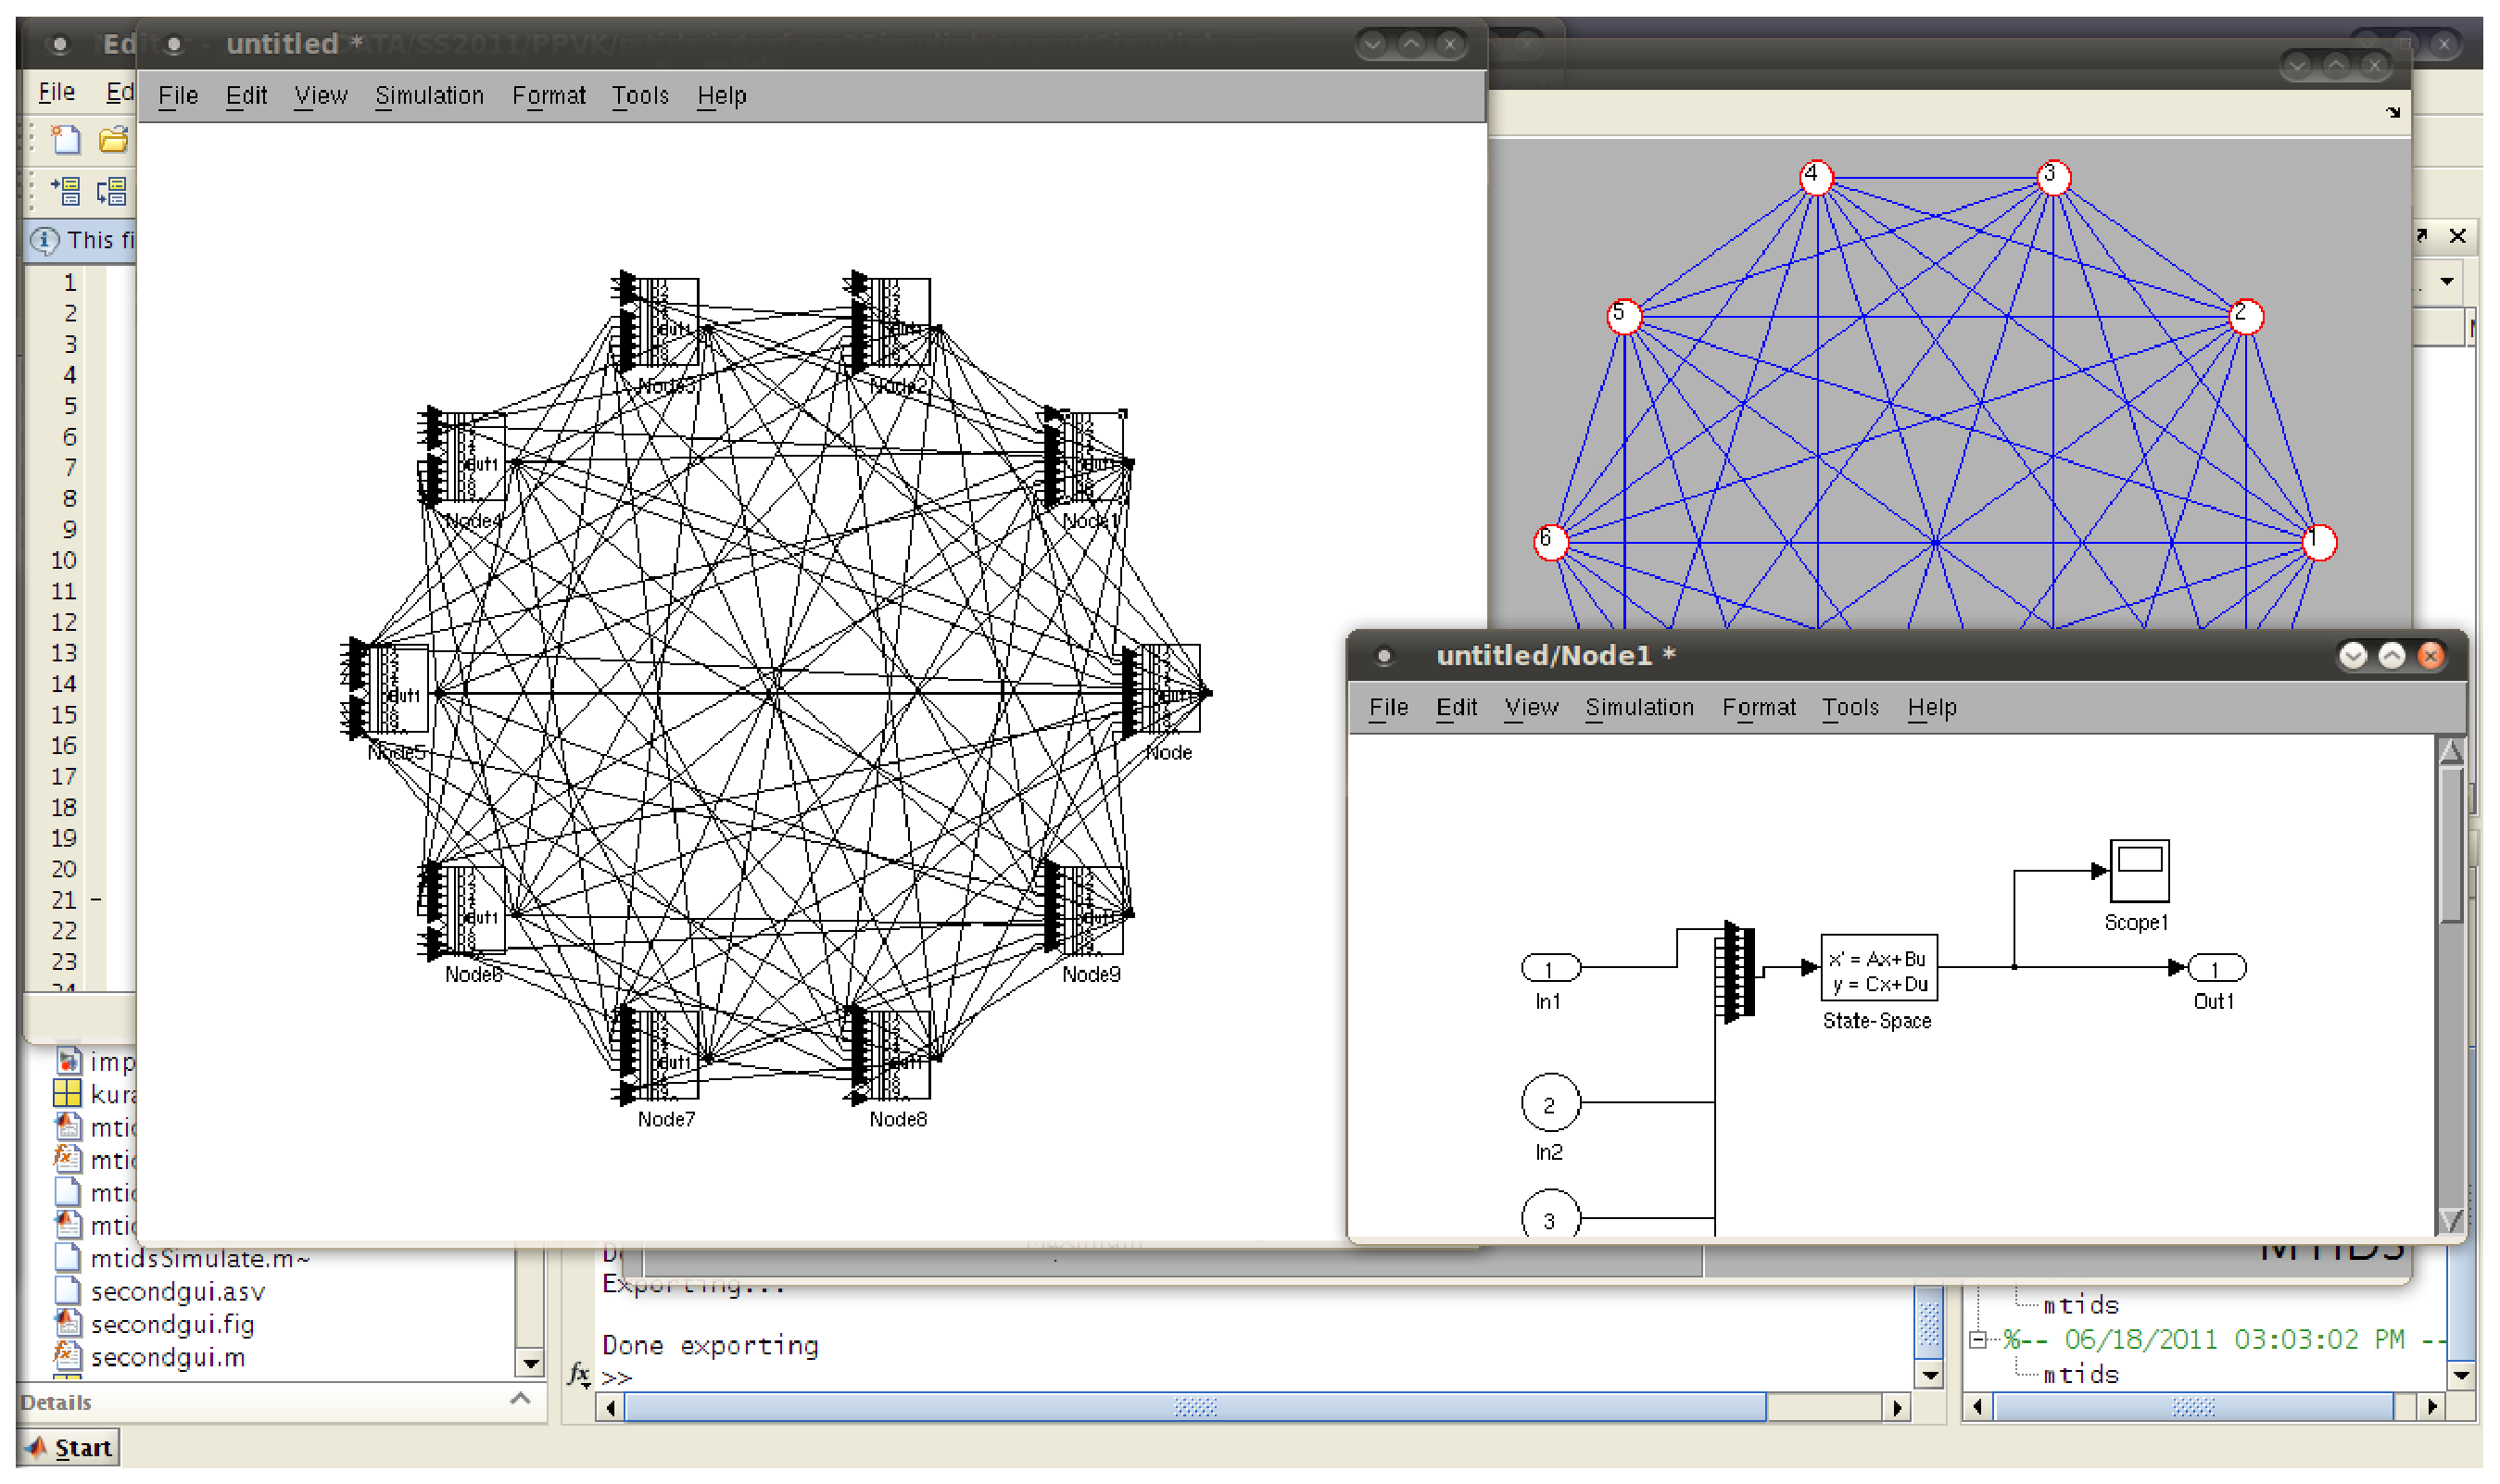
\includegraphics[width=0.9\textwidth]{pics/screenExportResult.eps}
\caption[MTIDS exported Simulink model]{Interconnected system Simulink Model. Example is a complete graph with 10 LTI nodes. }
\label{exportFig}
\end{figure}

In Figure \ref{exportFig}, the nodes are odered in a circle, the topology of the system defined in MTIDS remains. The circle arrangement is a 
design descition, made, in order to allow a better acces to the nodes. Each one of the nodes is a subsystem block. The dynamic of the nodes is defined inside
the subsystem block. Moreover, each node has a single out-port and N in-ports, where N is the number of nodes the whole system has. Each node on the 
system has its own in-port on each node, compare with a zoom on the first node of our example in Figure \ref{nodeFig}. Notice that the port corresponding to the nodes number
should always be free, e.g. the first node has an unconnected in-port 1, the second node an unconnected in-port 2, etc. 
In case that a loop of a node with itself is required we recommend doing this inside the subsystem/node. 
 

 

\begin{figure}[htb]
\centering
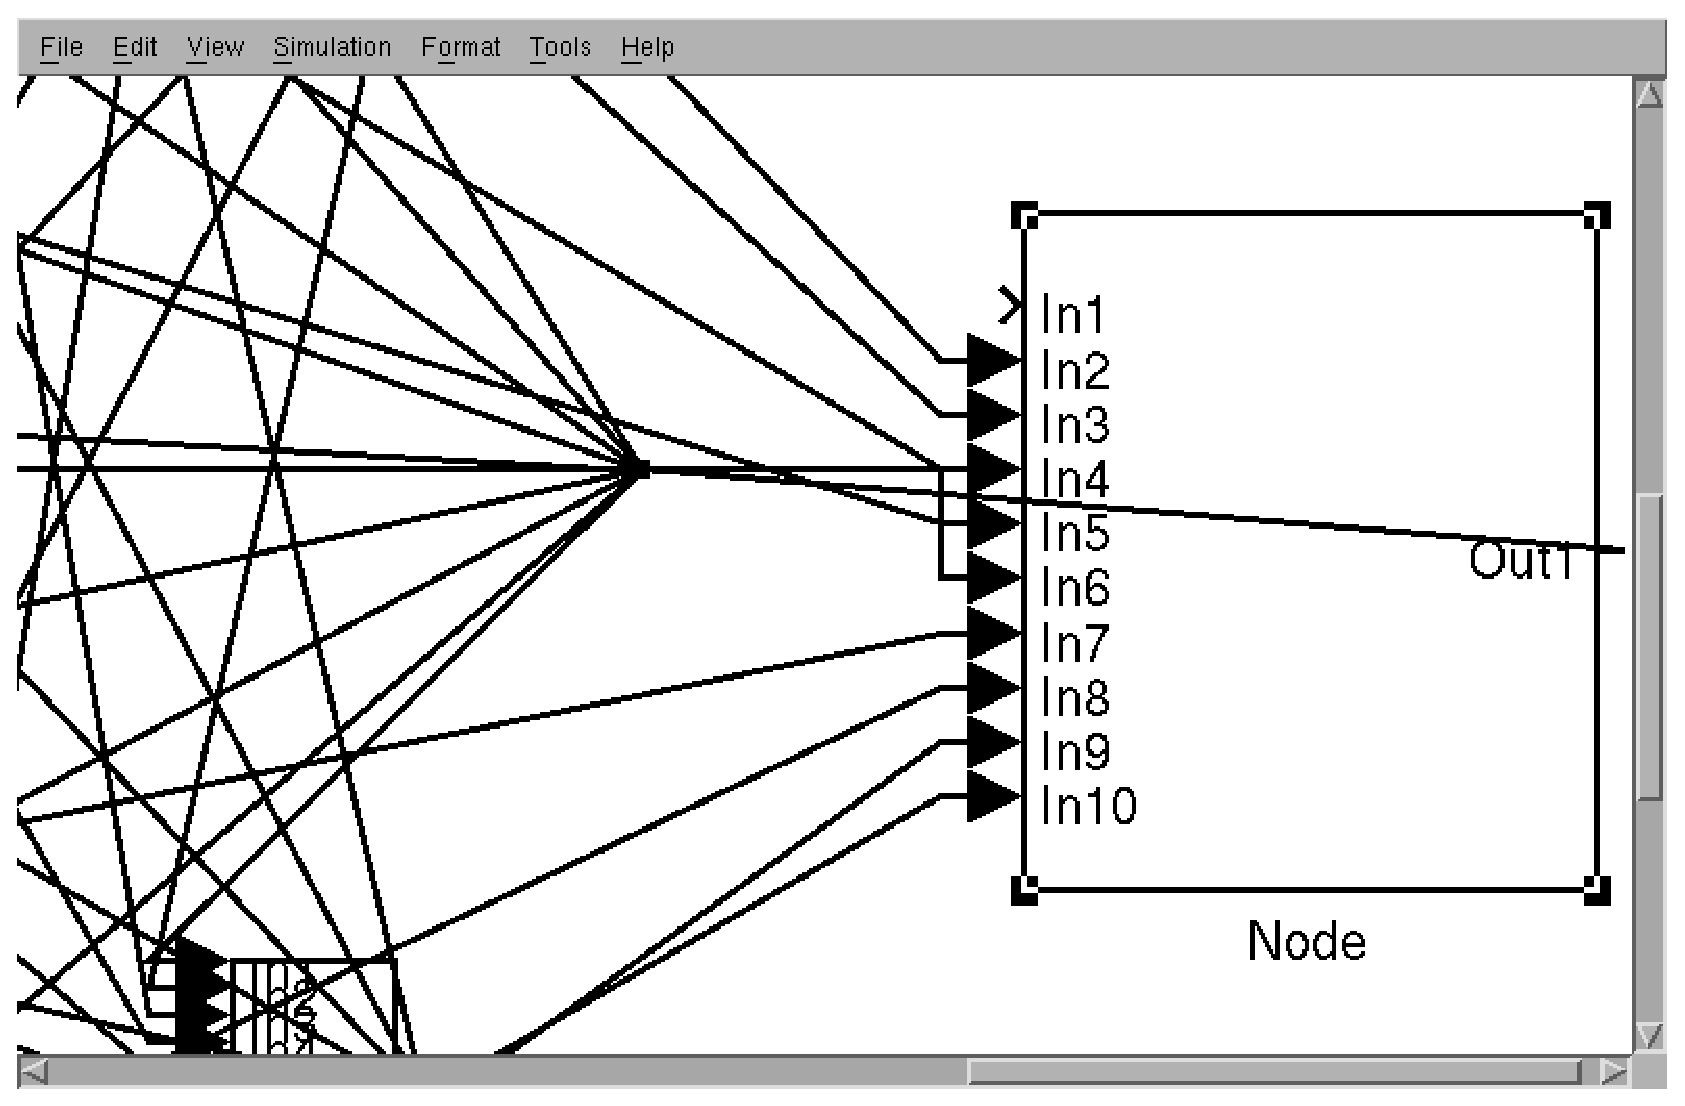
\includegraphics[width=0.7\textwidth]{pics/screenNode.eps}
\caption[MTIDS node in Simulink]{Node inputs and output: Each node has an in-port for every node in the model and an out-port. Example is the first node of a complete graph with 10 LTI nodes. }
\label{nodeFig}
\end{figure}

Another important aspect to point out is that when simulating the system, simulink will issue a warning for unconnected in-ports and set their input to the subsystem to 0, this means 
that an \textbf{unconnected ports enter the subsystem (local dynamics of the node) with a value of zero} during simulations. 

\section{Nodes' Dynamics}

As mentioned in the past section \ref{exportToSimulink} each node defined in MTIDS is exported to simulink as a subsystem. The exportSimulink.m function 
uses predefined dynamic templates, which are modified accourding to the in MTIDS defined topology. Next we explain how to define your own templates and
show how to use 2 preloaded templates: the LTI template and the kuramoto template. 


\subsection{Build your own Template}
The real power of MTIDS depends on you ability to build templates. 
\\
\begin{figure}[htb]
\centering
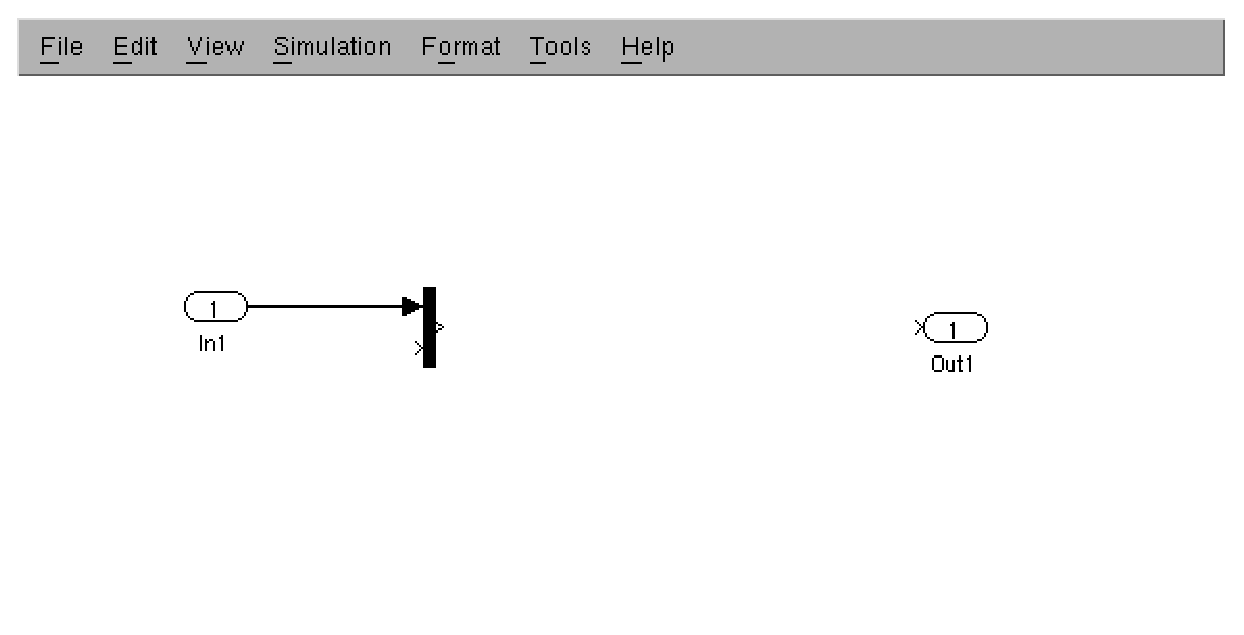
\includegraphics[width=0.6\textwidth]{pics/screenBuildTemplate.eps}
\caption[MTIDS Dynamics Template]{Scratch template for node's dynamics.}
\label{templateFig}
\end{figure}

In Figure \ref{templateFig} we can see the components that each template should have: an in-port connected to a mux and an out-port.
Between the mux and the outport you can design your own custom dynamics. The imput to the system comes from mux as vector composed by the values
send from other nodes/subsystems. The output of your system should also be aggregated to a vector and routed to the out-port. The sepparation of the different inputs and outputs 
is left to the system designers. With a well thought architecture complex systems are very easy to achieve, please refer to the LTI and kuramoto template examples.  
\\

The dynamic of a node can be as simple as a junction that only reroutes the incomming signals or more complicated to include controlers and systems inside of it. It is this feature that allows
the implementation of clusters or layered systems, see subsection \ref{layering}. 


\subsection{The LTI template}

The LTI template is an example that defines a linear time invariant dynamic for nodes. The mathematical model 
of a simple interconnected LTI system is written as:
\begin{eqnarray}
\left( \begin{array}{c}
\dot{x_1} \\  
\vdots \\
\dot{x_N}
\end{array} \right)=
\left( \begin{array}{ccc}
A_{11} & \cdots & A_{1N} \\  
\vdots & \ddots & \vdots\\
A_{N1} & \cdots &A_{NN}
\end{array} \right) 
\left( \begin{array}{c}
x_1 \\  
\vdots \\
x_N
\end{array} \right)+
\left( \begin{array}{c c c}
B_{1} & \cdots & B_{N}  
\end{array} \right) 
\left( \begin{array}{c}
u_1 \\  
\vdots \\
u_N
\end{array} \right)       
\end{eqnarray}
or
\begin{equation}
 \dot{x}=Ax+Bu
\end{equation}
The local view of a single subsystem/node (here for the first node) is:
\begin{eqnarray}
  \dot{x_1}= 
\left( \begin{array}{c c c c c c c}
A_{11} & A_{12} & \cdots & A_{1N} & B_{1} & \cdots & B_{N}  
\end{array} \right) 
\left( \begin{array}{c}
x_1 \\ 
x_2 \\ 
\vdots \\
x_N\\
u_1 \\  
\vdots \\
u_N
\end{array} \right)    
\end{eqnarray}
this can be reformulated  
\begin{eqnarray} \label{LTIFor}
 \dot{x_1}= A_{11}x_1 +  
\left( \begin{array}{c c c c c c c}
A_{11} & A_{12} & \cdots & A_{1N} & B_{1} & \cdots & B_{N}  
\end{array} \right) 
\left( \begin{array}{c}
0 \\ 
x_2 \\ 
\vdots \\
x_N\\
u_1 \\  
\vdots \\
u_N
\end{array} \right) 
\end{eqnarray}





In order to keep things simple, we define the local output of all nodes as:
\begin{eqnarray}
 y_N=  x_N 
\end{eqnarray}

To implement this dynamic as a template we make use of the State-Space block.

\begin{figure}[htb]
\centering
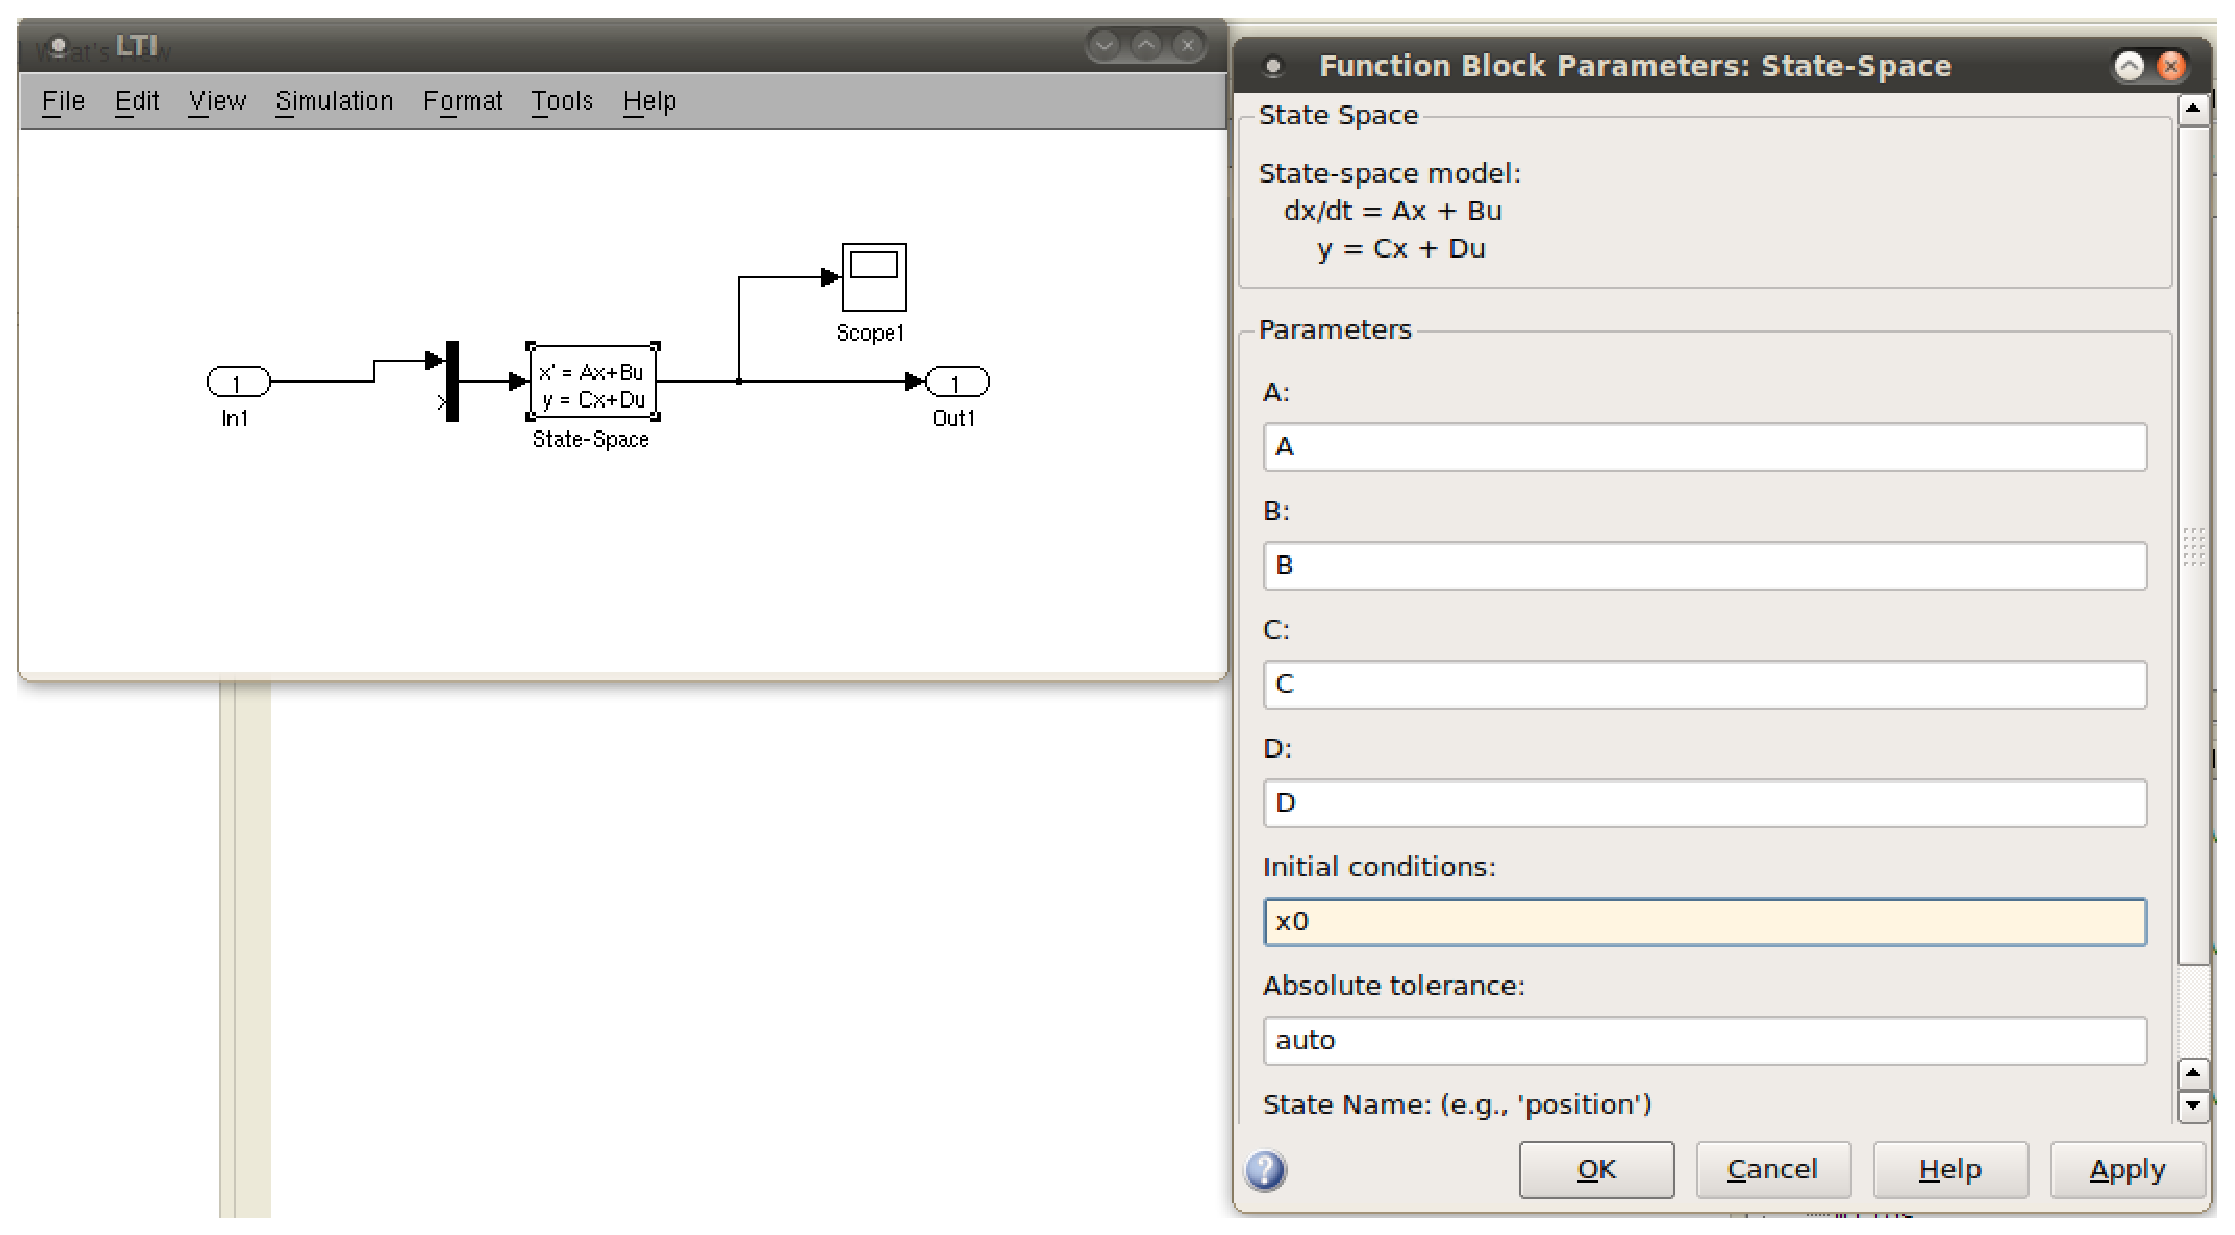
\includegraphics[width=0.8\textwidth]{pics/screenLTI.eps}
\caption[MTIDS LTI Template]{LTI template}
\label{templateLTIFig}
\end{figure}
 
This template shown in \ref{templateLTIFig} can be used in MTIDS to create interconnected LTI systems with different topologies. One way to avoid 
the work of parametrizing the A,B,C and D matrix of every node sepparately is to define the same matrix for all subsystems. One can use the formula 
\ref{LTIFor} and define the same A, B, C, and D matrix for every node. An example of this is
\begin{eqnarray}
 A&=& 1\nonumber\\
B&=&[1 \cdots 1]^{1\times N}\nonumber\\
C&=& 1\nonumber\\
D&=& [0 \cdots 0] ^{1\times N}\nonumber
\end{eqnarray}

As the in-port corresponding to the node itself is automatically set to zero by Symulink during the simulation, we can define the same matrizes for all 
nodes without getting any errors.
\\

For more complicated LTI models we recomend creating many different LTI templates.

\subsection{The Kuramoto Template}
The kuramoto template is an example for a non-linear dynamic of a node. 


\section{Layering/Clustering Nodes} \label{layering}



\section{Working in Simuling}



\section{Import from Simulink}

Beware to define nodes dynamics...


\chapter{Conclusion and Future Development}

\section{Conclusion}


\section{Future Development}
%
%_______________________________________________________________


%_____Abbildungsverzeichnis_________________________________
\cleardoublepage
\addcontentsline{toc}{chapter}{List of Figures} 
\listoffigures 	 %Abbildungsverzeichnis

%___________________________________________________________
% 
% %_____Literaturverzeichnis_________________________________
% \cleardoublepage
% \addcontentsline{toc}{chapter}{Bibliography}
% \bibliography{bibliography.bib}
% \bibliographystyle{alpha}
% %__________________________________________________________


%________________Appendix_____________________________________________%


\end{document}
